\documentclass[a4paper, 12pt]{report}
\usepackage{tikz}
\usepackage{pgfplots}
\usepackage{lipsum}
\usepackage{graphicx}
\newcommand{\italic}[1]{\textit{#1}}

\begin{document}
    \tableofcontents
    \section{Simple curve}
    This is a simple plot of $x^2$:
    \begin{center}
        \begin{tikzpicture}
            \begin{axis}[ axis lines = left, xlabel = $x$, ylabel = $f(x)$ ]
                \addplot[ domain = -10:10, samples = 5, color = blue ] {x^2};
            \end{axis}
        \end{tikzpicture}
    \end{center}
    \section{Change the axis}
    Is changed the axis:
    \begin{center}
        \begin{tikzpicture}
            \begin{axis}[ 
                axis x line = center,
                xlabel = $x$,
                xlabel style={above right},
                xmin = -5, xmax = 5, 
                axis y line = center,
                ylabel = $f(x)$,
                ylabel style={above left},
                ymin = -5, ymax = 5]
            \addplot[ domain = -5:5, samples = 100, color = blue ] {x^2};
            \end{axis}
        \end{tikzpicture}
    \end{center}
    You can correct the bug of the axis like this (acting to the xtick):
    \begin{center}
        \begin{tikzpicture}
            \begin{axis}[ 
                axis x line = center,
                xlabel = $x$,
                xlabel style={below right},
                xtick = {-4, -3,..., 3, 4},
                xmin = -1, xmax = 5, 
                axis y line = center,
                ylabel = $f(x)$,
                ylabel style={below left},
                ytick = {-4, -3,..., 3, 4},
                yticklabels={-4, -3,..., 3, 4,},
                ymin = -1, ymax = 5]
            \addplot[ domain = 0:2, samples = 100, color = blue ] { x^2 };
            \end{axis}
        \end{tikzpicture}
    \end{center}

    \section{Add a Grid}
    This the same plot with the grid:
    \begin{center}
        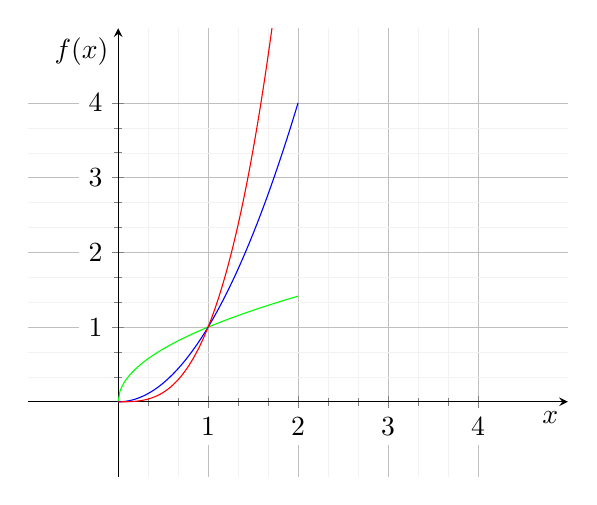
\begin{tikzpicture}
            \begin{axis}[ 
                axis x line = center,
                xlabel = $x$,
                xtick = {0, 1, 2, 3, 4},
                xticklabels={, 1, 2, 3, 4},
                xlabel style={below left},
                xmin = -1, xmax = 5, 
                axis y line = center,
                ylabel = $f(x)$,
                ylabel style={below left},
                ytick = {0, 1, 2, 3, 4},
                yticklabels={, 1, 2, 3, 4},
                ymin = -1, ymax = 5,
                ticklabel style={fill=white},
                grid = both,
                grid style={line width=.1pt, draw=gray!10},
                major grid style={line width=.2pt, draw=gray!50},
                minor tick num=2] 
            \addplot[ domain = 0:2, samples = 100, color = green ] {x^(1/2) };
            \addplot[ domain = 0:2, samples = 100, color = blue ] { x^2 };
            \addplot[ domain = 0:2, samples = 100, color = red ] { x^3 };
            \end{axis}
        \end{tikzpicture}
    \end{center}

	\section{Add the Legend}
	This the same plot with legend:
	\begin{center}
		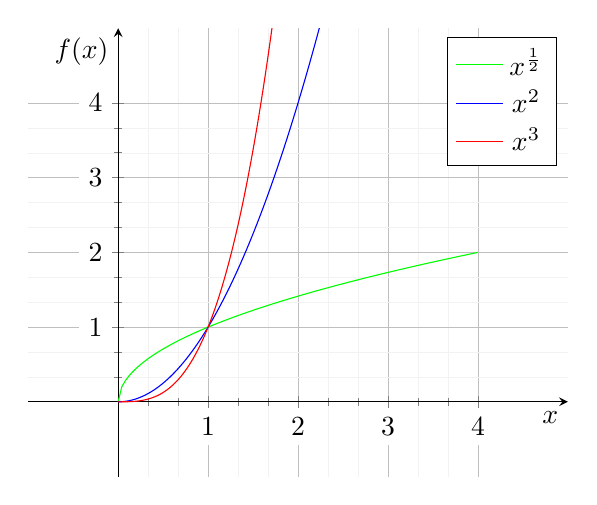
\begin{tikzpicture}
		\begin{axis}[ 
		axis x line = center,
		xlabel = $x$,
		xtick = {0, 1, 2, 3, 4},
		xticklabels={, 1, 2, 3, 4},
		xlabel style={below left},
		xmin = -1, xmax = 5, 
		axis y line = center,
		ylabel = $f(x)$,
		ylabel style={below left},
		ytick = {0, 1, 2, 3, 4},
		yticklabels={, 1, 2, 3, 4},
		ymin = -1, ymax = 5,
		ticklabel style={fill=white},
		grid = both,
		grid style={line width=.1pt, draw=gray!10},
		major grid style={line width=.2pt, draw=gray!50},
		minor tick num=2] 
		\addplot[ domain = 0:4, samples = 100, color = green ] { x^(1/2) };
		\addlegendentry{$x^{\frac{1}{2}}$}
		\addplot[ domain = 0:3, samples = 100, color = blue ] { x^2 };
		\addlegendentry{$x^2$}
		\addplot[ domain = 0:2, samples = 100, color = red ] { x^3 };
		\addlegendentry{$x^3$}
		\end{axis}
		\end{tikzpicture}
	\end{center}	
	\newpage
	\section{Importing from the pdf}
	I'm importing the image from pdf in order to apply a scale:
	\begin{figure}[!h]
		\centering
		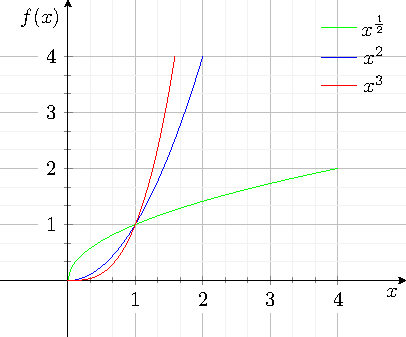
\includegraphics[scale = 1.7]{./images/simpleGraph/fig_1_1.pdf}
		\caption{Image generate with the import}
	\end{figure}
	
	\newpage
	
	\section{Fixing the border of the grid}
	This is the pre-def version of the graph:
	\begin{center}
		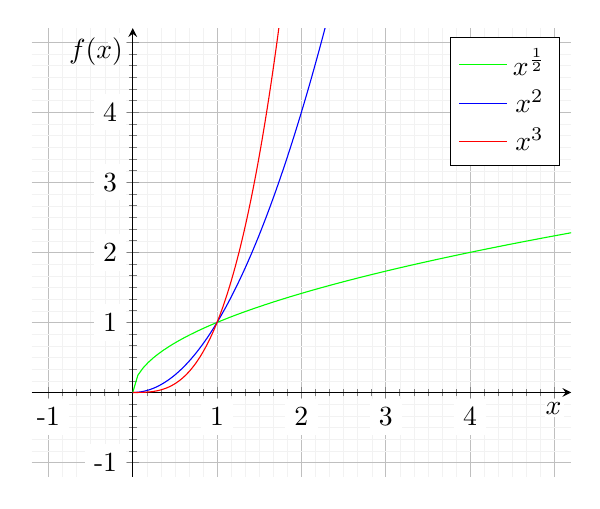
\begin{tikzpicture}
		\begin{axis}[ 
		axis x line = center,
		xlabel = $x$,
		xtick = {-1, 0, 1, 2, 3, 4, 5},
		xticklabels={-1, , 1, 2, 3, 4},
		xlabel style={below left},
		xmin = -1, xmax = 5, 
		axis y line = center,
		ylabel = $f(x)$,
		ylabel style={below left},
		ytick = {-1, 0, 1, 2, 3, 4, 5},
		yticklabels={-1, , 1, 2, 3, 4},
		ymin = -1, ymax = 5,
		ticklabel style={fill=white},
		grid = both,
		enlargelimits={abs=0.2},
		grid style={line width=.1pt, draw=gray!10},
		major grid style={line width=.2pt, draw=gray!50},
		minor tick num=5] 
		\addplot[ domain = 0:6, samples = 100, color = green ] { x^(1/2) };
		\addlegendentry{$x^{\frac{1}{2}}$}
		\addplot[ domain = 0:3, samples = 100, color = blue ] { x^2 };
		\addlegendentry{$x^2$}
		\addplot[ domain = 0:2, samples = 100, color = red ] { x^3 };
		\addlegendentry{$x^3$}
		\end{axis}
		\end{tikzpicture}
	\end{center}

	\section{Final version of the graph}
	This is, in my  opinion the final version of a plot:
	\begin{figure}[!h]
		\centering
		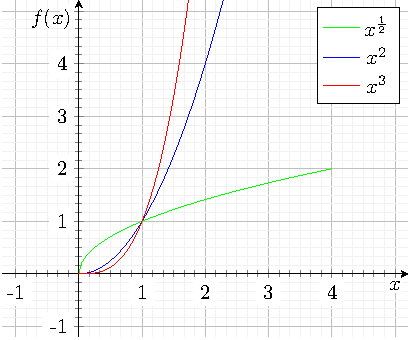
\includegraphics[scale = 1.7]{./images/defFig/fig_1_2.pdf}
	\end{figure}
\end{document}